%header and footer for separate chapter files

\ifx\whole\undefined
\documentclass[12pt, leqno]{book}
\usepackage{graphicx}
\input style-for-curves.sty
\usepackage{hyperref}
\usepackage{showkeys} %This shows the labels.
%\usepackage{SLAG,msribib,local}
%\usepackage{amsmath,amscd,amsthm,amssymb,amsxtra,latexsym,epsfig,epic,graphics}
%\usepackage[matrix,arrow,curve]{xy}
%\usepackage{graphicx}
%\usepackage{diagrams}
%
%%\usepackage{amsrefs}
%%%%%%%%%%%%%%%%%%%%%%%%%%%%%%%%%%%%%%%%%%
%%\textwidth16cm
%%\textheight20cm
%%\topmargin-2cm
%\oddsidemargin.8cm
%\evensidemargin1cm
%
%%%%%%Definitions
%\input preamble.tex
%\input style-for-curves.sty
%\def\TU{{\bf U}}
%\def\AA{{\mathbb A}}
%\def\BB{{\mathbb B}}
%\def\CC{{\mathbb C}}
%\def\QQ{{\mathbb Q}}
%\def\RR{{\mathbb R}}
%\def\facet{{\bf facet}}
%\def\image{{\rm image}}
%\def\cE{{\cal E}}
%\def\cF{{\cal F}}
%\def\cG{{\cal G}}
%\def\cH{{\cal H}}
%\def\cHom{{{\cal H}om}}
%\def\h{{\rm h}}
% \def\bs{{Boij-S\"oderberg{} }}
%
%\makeatletter
%\def\Ddots{\mathinner{\mkern1mu\raise\p@
%\vbox{\kern7\p@\hbox{.}}\mkern2mu
%\raise4\p@\hbox{.}\mkern2mu\raise7\p@\hbox{.}\mkern1mu}}
%\makeatother

%%
%\pagestyle{myheadings}

%\input style-for-curves.tex
%\documentclass{cambridge7A}
%\usepackage{hatcher_revised} 
%\usepackage{3264}
   
\errorcontextlines=1000
%\usepackage{makeidx}
\let\see\relax
\usepackage{makeidx}
\makeindex
% \index{word} in the doc; \index{variety!algebraic} gives variety, algebraic
% PUT a % after each \index{***}

\overfullrule=5pt
\catcode`\@\active
\def@{\mskip1.5mu} %produce a small space in math with an @

\title{Personalities of Curves}
\author{\copyright David Eisenbud and Joe Harris}
%%\includeonly{%
%0-intro,01-ChowRingDogma,02-FirstExamples,03-Grassmannians,04-GeneralGrassmannians
%,05-VectorBundlesAndChernClasses,06-LinesOnHypersurfaces,07-SingularElementsOfLinearSeries,
%08-ParameterSpaces,
%bib
%}

\date{\today}
%%\date{}
%\title{Curves}
%%{\normalsize ***Preliminary Version***}} 
%\author{David Eisenbud and Joe Harris }
%
%\begin{document}

\begin{document}
\maketitle

\pagenumbering{roman}
\setcounter{page}{5}
%\begin{5}
%\end{5}
\pagenumbering{arabic}
\tableofcontents
\fi


\chapter{Smooth plane curves and curves of genus 1}\label{3b}\label{genus 1 chapter}

If $C$ is a 
\index{curve of genus 1}%
curve of genus 1, then by Corollary~\ref{degree 2g+1 embedding}, any complete linear series $D$ of
degree $3 = 2g+1$ on $C$ is very ample. By the Riemann--Roch theorem any invertible sheaf
of degree $d>0$ on $C$ has $d$ sections, so the morphism associated to $D$ embeds $C$
as a plane curve of degree 3, on which $D$ is the intersection of $C$ with a line. 

We therefore begin this chapter with a general explanation of 
\index{sheaf of differentials}%
sheaves of differentials and linear
series on smooth plane curves, and use that theory to say a little about other embeddings of 
curves of genus 1. Though most curves cannot be realized as smooth plane curves, we shall see
in Proposition~\ref{nodal projection} that every curve can be
projected birationally to a plane 
\textit{nodal curve}
\index{nodal curve|defi}%
(that is, one having only ordinary nodes as singularities), 
and in Chapter~\ref{PlaneCurvesChapter} we will 
explain the analogous treatment of differentials and linear series on
such 
nodal curves, and more
generally\emdash but with less specificity\emdash on all reduced plane curves.

Using the plane model of a curve of genus 1, we shall see that the
theory is only a little more complicated than for genus 0. (But curves
of genus 1 over number fields 
occupy
many modern number theorists!)


\section{Riemann, Clebsch, Brill and Noether}
For a long time, 
\blue{plane curves}
\index{plane curve}%
were the only algebraic curves that were
studied. Originally these were curves in the affine plane over the
real numbers, but by the second half of the 
nineteenth
century the complex
projective plane was well understood, and curves in $\PP^2 =
\PP^2_\CC$, corresponding to irreducible forms in 3 variables, were
recognized as the natural objects of study (see Chapter \ref{Appendix-History}.)
\looseness=-1

The work of Bernhard Riemann dramatically changed the focus of the
\index{Riemann, Georg Friedrich Bernhard}%
theory to branched coverings of   
what we know as the Riemann sphere, or $\PP^1_\CC$.
The 
\blue{Riemann--Roch theorem,}
\index{Riemann--Roch theorem}%
in particular, gave
information about the existence of meromorphic functions on such
coverings, well beyond what could be done in the earlier theory.
However, Riemann's work, depending as it did on the then-obscure
\index{Dirichlet principle}%
``Dirichlet principle'', was not universally accepted. In the 1860s
\index{Clebsch, Alfred}%
\index{Brill, Alexander}%
\index{Noether, Max}%
Alfred Clebsch and, after the death of Clebsch  in 1872, Alexander
Brill and Max Noether (Emmy Noether's father) undertook the ambitious
program of redoing the Riemann--Roch theorem entirely in terms of
plane curves. They went beyond Riemann in certain directions, too: the
Brill--Noether theorem treated in our Chapter~\ref{Brill--Noether} was
formulated by Brill and Noether, and ``proved'' by them through an
unsupported general position assumption.

A central difficulty in the Brill--Noether attempt on the Riemann--Roch theorem was that,
although any smooth curve can be embedded in $\PP^r$ for any $r \geq 3$, most curves cannot be embedded in the plane. 
However, as is shown in Section~\ref{good projections}, we can embed
$C$ as a curve $ C \subset \PP^r$ in a higher-dimensional projective
space and find a projection $\PP^r \to \PP^2$ that carries $C$
birationally onto its image $C_0$, called a 
\blue{plane model}
\index{plane model}%
of $C$. The
curve $C_0$ typically has singularities, and $C$ is the normalization
of $C_0$. Brill and Noether wanted to prove the Riemann--Roch theorem
for $C$ by formulating and proving a related theorem for $C_0$. In
particular, they tried to characterize 
\blue{linear equivalence of divisors}
\index{linear equivalence of divisors}%
\index{clusters of points}%
on $C$ in terms of certain ``clusters'' of points\emdash we would say
0-dimensional subschemes\emdash of $C_0$.  

To carry out this program, a key step was to show that if $D\subset C_0$ is contained in the intersection
$D'$ of $C_0$ and some other plane curve $C_0'$, then a divisor 
$E \colonequals D'-D$ can be defined with properties such as that $D'-E = D$;
Brill and Noether seem simply to have assumed that this is so. A bit
\index{Macaulay, Frances Sowerby}%
later Frances Sowerby Macaulay proved that this is in fact possible
and also understood that it would not generally be possible if $D'$
were the intersection of three or more curves.
(In modern terms, the intersection of two curves is 
\index{Gorenstein}%
\blue{Gorenstein;}
the intersection of 3 is generally not.)

Macaulay exploited this theory of 
\blue{residuation}
\index{residuation}%
to prove what he called
the generalized Riemann--Roch theorem
\index{generalized Riemann--Roch theorem}%
\index{Riemann--Roch theorem!generalized}%
(Theorem~\ref{CBM}). This
early work of Mac\-aulay led directly to his definitions of
\index{perfect ideal}%
``perfection'' (a homogeneous ideal 
$I  \subset S\colonequals k[x_0, \dots, x_n]$ is perfect if $S/I$ is 
\blue{Cohen--Macaulay)}
\index{Cohen--Macaulay}%
and ``super-perfection'' (the case when $S/I$ is
\index{super-perfect ideal}%
\index{Gorenstein}%
Gorenstein). For all this, see \cite{eisenbud-gray}.

In this section we will take the point of view of Clebsch, Brill and Noether, and explain how to understand 
the differential forms and, given a (possibly ineffective) divisor $D$ on $C$, how to find all the 
effective divisors on $C$ that are linearly equivalent to $D$, in terms of a smooth plane curve. In Chapter~\ref{PlaneCurvesChapter} we will return to this point of view and treat the case of
nodal curves and the case of arbitrary reduced plane curves. We will give effective algorithms for
two constructions:

\begin{enumerate}
\item Given the equation $F(X,Y,Z)$ of a smooth $d$ plane curve $C$
of degree $d$, we can
construct a basis for $H^0(K_C)$. 
\item  Given a possibly ineffective divisor $D = D_{+}-D_{-}$ on $C$ we can construct the complete linear series $|D|$ on $C$. In particular we can:
\begin{enumerate}
\item determine whether $D$ is equivalent to any effective divisor on $C$; and if so,
 \item find all effective divisors $E$ on $C$ with $E \sim D$;
 \item find a basis of $H^0(\cO_C(D))$, expressed in terms of curves of high degree with  
\index{base locus}%
base locus;
 \item find the homogeneous coordinate ring of the morphism defined by $|D|$ or a subseries.
\end{enumerate}
\end{enumerate}

\section{Smooth plane curves}\label{smooth plane curves}

\subsection{Differentials on a smooth plane curve}\label{canonical series on smooth plane curves}

Let $C \subset \PP^2$  be a smooth plane curve, given as the zero locus of a homogeneous polynomial $F(X,Y,Z)$ of degree $d$. By the 
\blue{adjunction formula}
\index{adjunction formula}%
(Proposition~\ref{adjunction}) the canonical  divisors on $C$
are the intersections of $C$ with curves of degree $d@{-}@3$. In the spirit of Brill and Noether we
will make this explicit by constructing all
 the 
regular differential forms
\index{regular differential forms}%
\index{differential forms!regular}%
 on $C$ in terms of forms of degree $d@{-}@3$.

For this purpose we introduce coordinates $x = X/Z$ and $y = Y/Z$ on the affine open subset $U \cong \AA^2$ given by $Z \neq 0$, and let $f(x,y) = F(x, y,1)$ be the inhomogeneous form of $F$, so that $C^\circ = C \cap U$ is the zero locus $V(f) \subset  \AA^2` `$. 

Since an automorphism of $\PP^2$ can carry any point in $\PP^{2}$ to any other point, we may assume
that 
the point $[0,1,0]$ (that is, the point at infinity
in the vertical direction) does not lie on $C$, so that the
 projection  $\pi: C \to \PP^1$ from $(0,1,0)$, which is given by $[X,Y,Z] \mapsto [X,Z]$ (or, in affine coordinates, $(x,y) \mapsto x$)  has degree $d$. Let $D$ be the divisor defined by the intersection of $C$ with the line $Z=0$ at infinity.

Consider the
regular 1-form $dx$ on $\AA^2` `$, which we may regard as the pullback of the form $dx$ on
 $\AA^{1}$.
Since the form $dx$ on $\PP^{1}$ has a 
\index{double pole}%
double pole
at infinity the form $dx|_{C}$ has polar
locus $2D$.
 
 \def\Co{{C^{\circ}}}
How do we get rid of the poles of $dx$? The extension to $\PP^2$ of a polynomial $h(x,y)$ of degree $m$ on
$\AA^2$ has a pole of order $m$ along the line $L$ at infinity. Thus if $h$ has degree at least 2 then $dx/h$ has no poles at infinity. However, $h(x,y)$ may well vanish at points of $\Co$, and this may create new poles of $dx/h$. Of course if $h$ vanishes only at  points of $\Co$ where $dx$ has a zero, the zeroes of $h$ may cancel the zeroes of $dx$ rather than creating new poles.
 
 To avoid producing new poles in this way we may take
 $$
 h(x,y) = f_{y} \colonequals \frac{\partial f}{\partial y}(x,y).
 $$
 We claim that 
 $$
\varphi_0 = \frac{dx}{f_{y}}
$$
is everywhere regular and nowhere 0 in $C^\circ$. 

Note that $df$ vanishes identically when restricted to $C^\circ$, so
 $$
 0 \equiv df|_{\Co} = f_{x}dx|_{\Co} + f_{y}dy|_{\Co} .
 $$
Clearly $\varphi_0$ is regular at points $p$ where
$f_{y}(p) \neq 0$. At such a point, if $dx|_{\Co}$ were 0, then since
$\Co$ is smooth we would have $dy|_{\Co} \neq 0$, contradicting the
equation above. Thus $\varphi_{0}$ is both regular and nonzero at such
points. On the other hand, if $f_{y}(p) = 0$, then since $\Co$ is
smooth at $p$
we also have $f_{x}(p)\ne0$, 
so $dx|_{\Co}$ and $f_{y}$ vanish to the same
order, whence, again, $\varphi_0 = (dx/f_{y})|_{\Co}$ is regular and nonzero, proving the claim.

Put differently, if $L$ is the line at infinity, so that $U = \PP^{2}\setminus L \cong \AA^{2}$,
\index{cotangent bundle}%
then the cotangent bundle on $U$ is 
$\Omega_{U}=\sO_{U}dx \oplus \sO_{U}dy$,
so 
the cotangent bundle $\Omega_{\Co}$ on $C^{\circ}$, which is the canonical bundle $\omega_{\Co}$,
 is the cokernel of the map from the normal sheaf $\sO_{C}(-d)|_{U}$ to the restriction of 
$\Omega_{U}$ to $C^{\circ}$. This map sends the local generator $f$ of the normal sheaf to
$f_{x}\,dx+f_{y}\,dy \in \Omega_{U}$, and because $f_{x}$ and $f_{y}$
have no common zeros, the generator $d_{y} \in \Omega_{C^{\circ}}$
is a multiple of $dx/f_{y}$.
Thus the free $\sO_{C^{\circ}}$-module $\omega_{C}|_{C^{0}}$ is generated by $dx/f_{y}$.

Since $f_{y}$ has degree $d@{-}1$, the rational function $1/f_{y}$ vanishes to order $d@{-}1$ on the line
at infinity, and thus in particular on the divisor $D$. Thus $\varphi_0$ vanishes to order $d@{-}@3$ on $D$; in other words, as divisors,
$$
(\varphi_0) = (d@{-}@3)D.
$$
In particular, if $d \geq 3$ then $\varphi_0$ is a globally 
\index{regular differential}%
on $C$. The divisor of
zeros of this differential has degree $d(d@{-}@3)$. If $g$ is the
genus of $C$, then 
$2g-2 = d(d@{-}@3)$, whence 
\vspace*{-2pt}
$$
g = \frac{d(d@{-}@3)}{2} + 1 = \mbinom{d@{-}1}{2}.
\vspace*{2pt}
$$
We can produce a vector space of $\tbinom{d@{-}1}{2}$ regular differentials by multiplying $\varphi_0$ by 
polynomials $e(x,y)$ 
  of degree $d@{-}@3$, since this does not introduce any poles. This proves:

\begin{theorem}
The space of regular differentials on a smooth plane curve $C$
with affine equation $f=0$ is 
$$
\left\{ \frac{e(x,y)\,dx}{f_{y}} \biggm|\hbox{e(x,y) is a polynomial degree 
at most
$d@{-}@3$}\right\}.
\eqno{\qed}
 $$
\end{theorem}

\subsection{Linear series on a smooth plane curve}\label{linear series on smooth plane curves}

Any divisor on a smooth plane curve $C$ may be expressed as the difference of
\index{effective divisor}%
two 
effective divisors,
$D`=` D_{+}`-\nobreak D_{-}$. We would like to find all the \emph{effective} divisors 
\index{linearly equivalent}%
linearly equivalent
to $D$, that is, of the form
$D + (H/G)$, where $G, H$ are forms of the same degree $m$. We begin by choosing
an integer $m$, large enough so there is a form $G$ of degree $m$ vanishing on $D_+$ but not on all of $C$, so
that the divisor of zeros of $G$ is $A+D_+$ for some divisor $A$ on $C$.

\begin{theorem}\label{equiv on smooth plane curve}
Let $D= D_{+}-D_{-}$ be a divisor on 
a
smooth plane curve $C$. If
there is a form $G$ of degree $m$ vanishing on $D_{+}$ but not on all of $C$
then we may write $(G) = D_{+}+A$, and then
the effective divisors equivalent to $D$, if any, are precisely those 
of the form $(H) - A -D_{-}$, where $H$
is a form of degree $m$ vanishing on $D_{-}+A$, but not on all of $C$.
\end{theorem}

See Figure~\ref{Fig14.3} for an illustration with $D_+ = r+s+t, \ D_- = u$.
In particular, if no homogeneous polynomial $H$ of degree $m$ vanishes on  $A + D_{-}$ but not on $C$, then $D$ is not linearly equivalent to any effective divisor. The existence of such an $H$ is thus independent of the choices of $m$ and $G$, as we shall see in the proof.

The simplest special case of the theorem is the completeness
\index{complete linear series}%
of the linear series defined
by intersections of $C$ with curves of a given degree, 
or, equivalently, the fact that the restriction maps
$$
H^{0}(\sO_{\PP^{n}}(m)) \to H^{0}(\sO_{C}(m))
$$
are surjective for all $m$. 

\begin{proposition}\label {completeness of hyperplanes on plane curve}
If $C$ is a smooth plane curve, then any Cartier divisor on $D$ that is linearly equivalent to the divisor of
a form of degree $m$ is itself the divisor of a form of degree $m$; that is, plane curves are
\blue{arithmetically Cohen--Macaulay.}
\index{arithmetically Cohen--Macaulay}%
\end{proposition}

 The results for singular curves explained in Chapter~\ref{PlaneCurvesChapter}
 depend on strengthenings  of this condition.
 
\begin{proof}
Let $C$ be the plane curve defined by $F=0$, and let $D$ be the divisor on $C$ defined by a form $L$
of degree $m$, not vanishing on (any component of) the curve $C$. If $G$ and $H$ are forms of the same degree $t$, 
not vanishing on any component of $C$,
and $D+(G/H)$ is effective, then the divisor $(LG)$  on $C$ must contain the divisor $(H)$ on $C$.
This means that the subscheme of $\PP^{2}$ defined by $(LG,F)$ contains the scheme defined 
by $(H,F)$. Since $H$ and $F$ have no components in common, Theorem~\ref{Lasker} implies
that $LG = AH+BF$  for some forms $A,B$ with $\deg A = \deg LG -\deg H = m$,
 whence $D+(G/H) = (A)$
as required.
\end{proof}

\begin{example}
Suppose that $C$ has degree 3 and thus genus 1. If we choose as origin on the curve $C$ a point $o$, then to add two points $p$ and $q \in C$ means to find the (unique) effective divisor of degree 1 linearly equivalent to $p + q - o$. In this situation, Theorem~\ref{equiv on smooth plane curve} applies with $m=1$: there is a line $L$ 
containing $p+q$ defined by a linear form $G$. If $r \in C$ be the remaining point of intersection of $L$ with $C$ we can choose a linear form $H$ vanishing on $o+r$, and the line it defines meets $C$
in one additional point $s$. This is the classical construction of the 
\index{group law}%
group law
on the points of $C$ (or,
for curves over a field that is not algebraically closed, on the rational points of $C$).
See Figure~\ref{group law on cubic}.
\end{example}

\begin{proof}[Proof of Theorem~\ref{equiv on smooth plane curve}]
First, suppose that we can find a form $H$ of degree $m$ as in the theorem.
Setting $D' = (H) -(D_{-}+A)$ we have
$$
D' = D + (H/G) = D_{+}- D_{-} - (D_{+}+A)+(D_{-}+A+D')
$$
so $D'$ is linearly equivalent to $D$. 

\begin{figure}
\centerline{\includegraphics[height=1.15in]{"main/Fig14-1"}}
\nointerlineskip
\vskip-15pt
\centerline{\color{white} \vrule width 100pt height 12pt}
\vskip-3pt
\caption{If $G$ and $H$ have the same degree, then $r+s+t-u\sim p+q$ on $C$.}
\label{Fig14.3}
\end{figure}

We claim that we find in this way all effective divisors $D' \sim D$. 
To see this, suppose $D'$ is any effective divisor with $D' \sim D$, so that
$$
\cO_C(A+D_{-}+D') = \cO_C(A+D_{-}+D)  = \cO_C(m),
$$
that is, $A+D_{-}+D' \equiv (G)$ for some form $G$ of degree $m$. By Proposition~\ref{completeness of hyperplanes on plane curve}
this implies that $A+D_{+} = (H)$ for some form of degree $m$, as required.
\end{proof}


The argument given in Proposition~\ref{equiv on smooth plane curve} can be stated more generally thus:  if curves $F(X,Y,Z)=0$ and $Q(X,Y,Z)=0$ 
meet only in a finite set of points $\Gamma$ in $\PP^{2}$, and $E(X,Y,Z) = 0$ is a curve containing the intersection in an appropriate sense,
then $E = QH +LF$ for some forms $H$ and $L$, and this statement
applies to arbitrarily singular curves. Recognizing its importance for
the argument above and the generalizations to come, Max Noether
\index{Noether, Max}%
in \cite{Noether1873} dubbed it the \emph{fundamental theorem},
\index{fundamental theorem}%
noting that it had often been used by geometers but not proven. After successive attempts and 
\index{Brill, Alexander}%
criticisms involving many mathematicians, he and Brill gave a complete
proof in \cite{Brill-NoetherOriginal}. For more of this story see the
account in \cite{eisenbud-gray}.

\subsection{The Cayley--Bacharach--Macaulay theorem}\label{CB section}

The following result was proven by Macaulay \cite[p.~424]{Macaulay1900}, as a version of the Riemann--Roch theorem. It is now widely referred to as the Cayley--Bacharach theorem, named for an
\index{Macaulay, Frances Sowerby}%
\index{Cayley--Bacharach--Macaulay theorem}%
incorrect version asserted by Cayley and a correct special case later proved by
Bacharach \cite{Bacharach1886}; see \cite[Section 2.3]{eisenbud-gray} for more on this history, and 
\cite{MR1376653} (where the result is incorrectly attributed to Bacharach) for generalizations and related conjectures. Here is the version for divisors on a smooth plane curve:

\begin{theorem}[Cayley--Bacharach--Macaulay]\label{CBM} Let $C$ be a smooth plane curve of degree $d$, and suppose that
$E', E''$ are effective divisors on $C$ such that $E\colonequals E'+E'' = C\cap C'$, the complete intersection of $C$
with a curve $C'$ of degree $d'$. For any integer 
$\,0\leq k \leq d+d'-3$, the difference in the number of conditions imposed 
on forms of degree $k$ by $E''$ and by $E$ is equal to the degree of $E'$ minus the
number of conditions $E'$ imposes on forms of degree 
$d''\colonequals d+d'-3 -k$\emdash that is, the failure of
$E'$ to impose 
\blue{independent conditions}
\index{independent conditions}%
on forms of degree $d''$.

 Writing $H$ for
the divisor class on $C$ of the intersection of $C$ with a line, and setting $s \colonequals d+d'-3-k$, this is the equality
$$
h^0(kH-E) - h^0(kH-E')  = \deg E'' - \left(h^0(sH) -  h^0(sH-E'')\right)
.
\unif
$$
\end{theorem}

\begin{proof}
Set $e' \colonequals \deg E', \ e''\colonequals \deg E''$ and $e = e'+e'' = \deg E.$
By the adjunction formula, the divisor class of the canonical bundle
on $C$ is $K = (d-3)H$. Using the Riemann--Roch theorem, the left side
of the equality is 
$$
kd-e-h^0(K - (kH-E)) - \left(kd-e' - h^0(K-(kH-E'))\right).
$$
Since $K - (kH-E) = K - (kH-d'H) = sH$ and  $K-(kH-E') = sH+E''$, we see that the 
left side is equal to 
$
e'' - h^0(sH) +  h^0(sH+E'')
$
as required.
\unif
\end{proof}

As noted in \cite{eisenbud-gray}, the converse, proving the Riemann--Roch theorem for $C$ from Theorem~\ref{CBM}, is also easy.

\begin{corollary}\label{CBM cor 1}
A divisor $E'$ on a smooth plane curve $C\subset \PP^2$ of degree $d$ moves
in a linear series of dimension $r$ if and only if $E'$ fails by $r$ to impose
independent conditions on curves of degree $d-3$.
\unif
\end{corollary}

\begin{proof}
For sufficiently large $d'$ we can choose a curve $C'$ of degree $d'$ containing
$E$ and meeting $C$ in $E = E'+E''$, where $E''$ is disjoint from $E'$. Since $C\cap C'$
is a complete intersection, every form vanishing on $E+E'$ is a linear combination of
the forms defining $C$ and $C'$, and thus the dimension of the space of forms of degree $d'$
vanishing on $E$ modulo those vanishing on $C$ is~1. By
Theorem~\ref{equiv on smooth plane curve} the dimension $r$ of the
linear series $|E'|$ is the dimension of the space of
forms of degree $d'$ modulo those vanishing on $E+E'$, and by Theorem~\ref{CBM} this
is the failure of $E'$ to impose independent conditions on forms of degree
$d'' = d+d' - d' -3 = d-3$.
\unif
\end{proof}

To apply Theorem~\ref{CBM} it is helpful to know when points impose independent conditions on forms of a certain degree. Here is a first result of this kind:
\index{independent conditions!imposition by points}%

\begin{proposition}\label{n-2 independence}
Suppose that $1\leq n$. Any set $\Gamma$ of $k\leq n$ distinct points
in $\PP^{2}$ imposes independent conditions on forms of degree $n-1$;
and if $\,\Gamma$ is not contained in a line then $\Gamma$ imposes
independent conditions on forms of degree $n-2$.
\unif
\end{proposition}

\begin{proof} To show that $\Gamma$ imposes independent conditions on forms of degree $d$ we must produce, for each $p\in \Gamma$, a form of degree $d$ vanishing on 
$$
\Gamma_{p}\colonequals\Gamma\setminus\{p\}
$$
 but not $p$. If $\Gamma$ imposes independent conditions on forms of degree $d$ then
 $\Gamma$ automatically imposes independent conditions on forms of degree $d+1$,
 so we may assume that $k=n$.
 
The product of linear forms
 vanishing on general lines through the points of $\Gamma_{p}$ does not vanish at $p$, proving the first statement.

Now assume that $\Gamma$ is not contained in a line and $p\in \Gamma$.
It suffices to show that for each $p\in \Gamma$ there is a form of
degree $n-2$ vanishing on $\Gamma_{p}$ but not on $p$. Since $\Gamma$
spans $\PP^2` `$, there is a spanning set of three points $p,q,r$ of
$\Gamma$. The union of the line spanned by $q,r$ with general lines
through the $n-3$ points of $\Gamma_{p}\setminus\{q,r\}$ is defined by a form of degree $n-2$ containing $\Gamma_{p}$ but not $p$, 
as required. 
\end{proof}

\begin{corollary}\label{CBM cor 2}
 Suppose that $C\subset \PP^2$ is a smooth plane curve of degree $d\geq 3$.
 
\begin{enumerate}
 \item If $\,\sV$ is a $g^1_e$ on $C$ with $e\leq d-1$ then $e = d-1$ and $\sV$
 corresponds to projection from a point of $C$.
 \item If $\,\sV$ is a $g^2_e$ on $C$ with $e\leq d \geq 4$ then $e = d$. Furthermore,  the
  embedding of $C$ in $\PP^2$ is unique up to automorphisms of $\PP^2` `$.
 \end{enumerate}
\end{corollary}

\begin{proof}
(1) If $E$ is a divisor in the linear series $\sV$ then by Corollary~\ref{CBM cor 1} the points of $E$ fail to impose
 independent conditions on forms of degree $d-3$. By Proposition~\ref{n-2 independence} the degree of $E$ is $d-1$
 and the points lie in a line $L$, which must meet $C$ in an additional point $p$. By Theorem~\ref{equiv on smooth plane curve}
 the linear series $|E|$ is residual to $p$ in curves of degree 1; that is, it is the linear series corresponding to projection from $p$.
 
(2) In this case a divisor in the series $\sV$ fails by 2 to impose independent conditions on forms of degree $d-3$, and
 thus fails (by at least 1) to impose independent conditions on forms of degree $d-2$. By 
  Proposition~\ref{n-2 independence} the degree of $E$ is $d$.
 Moreover, the points lie in a line $L$; thus $\sV$ is a subseries of the series by which $C$ is embedded.
 \end{proof}

\section{Curves of genus 1 and the group law of an elliptic curve}

We will describe the maps of a curve of genus 1 given by
the complete linear series in the lowest degree cases of interest: $d =  2, 3, 4$ and $5$. Along the
way we will see several ways of parametrizing the family of curves of genus 1 by one-dimensional varieties,
\index{moduli space}%
forerunners of the moduli spaces that we will introduce in Chapters~\ref{ModuliChapter} and~\ref{CurvesModuliChapter}.


On a smooth, irreducible curve $E$ of genus 1 the canonical sheaf has degree~0;
and since it has a 
\index{global section}%
\blue{global section,}
it must be $\sO_C$.
Since invertible sheaves of negative degree cannot have 
nonzero sections,
\blue{the Riemann--Roch theorem}
\index{the Riemann--Roch theorem}%
shows that
$h^0( \sL) = \deg \sL$ for any $\sL$ of positive degree. Among the surprising consequences is that, given
\index{abelian algebraic group}%
a point $o\in E$, there is a natural structure of abelian algebraic group on the points of $E$ for which $o$
is the zero element. A curve of genus 1 with a chosen point $o$ is called an \emph{elliptic curve}.
\index{elliptic curve}%

\begin{proposition}\label{group law} Let $E$ be a curve of genus 1 and let $o$ be a chosen point $o\in E$.
If we set $p+q = r$, where $r$ is the unique effective divisor
linearly equivalent to $p+q-o$, then $E$ becomes a
commutative algebraic group.
Moreover, the group of divisor classes is 
\blue{divisible,}
\index{divisible group}%
in the sense that for any divisor $D$ of degree $n>0$
 there is a point $p$ such that $D\sim np$.
\unif
 \end{proposition}

\begin{proof}
 The group operation is easy to describe:
Let $E$ be an elliptic curve with the point $o\in E$ chosen arbitrarily. If $p,q$ are points of $E$ then $\sO_E(p+q-o)$ has degree 1, and
thus has a unique global section. This vanishes at a unique point $r$, which may also be described as the unique
effective divisor linearly equivalent to $p+q-o$, and thus 
$p+q = r$ in the group operation, which is thus obviously commutative. For the inverse, if $r$ is the  unique point
linearly equivalent to $2o-p$ then $p+r-o\sim o$, so that $r=-p$. For any divisor $D$
we define 
\index{notation!$\Sigma D$}%
\blue{$\Sigma D$}
to be the unique point linearly equivalent to $\Sigma D-(\deg D-1)o$.
In this group operation any two linearly
equivalent divisors have the same sum $\Sigma D = \Sigma D'$.

We can determine the point $r\sim p+q-o$ and show that the group law
is given by 
\blue{regular functions}
\index{regular function}%
as follows. By Corollary~\ref{degree 2g+1 embedding} we may embed $E$ in $\PP^2$ by any linear series
of degree 3.  Let $L$ be the line through $p+q$, and suppose that
$L$ meets $C$ in an additional point $s$. Since $s$ is unique, its coordinates are functions
\blue{polynomial functions}
\index{polynomial function}%
(on a suitable affine chart) of the coordinates of $p$ and $q$. The line through $s$ and $o$ meets $C$ additionally in a point $r$,
and by Theorem~\ref{equiv on smooth plane curve} we have $r\sim p+q-o$, as in Figure~\ref{group law on cubic}.
and similarly the point $r$ is a polynomial function of the coordinates of $s$ and $o$.

To see that $E$ is a divisible group, consider the maps $n: E\to E$ given by multiplication by integers $n$. Since the
group law is given by polynomial functions, the number of solutions $p$ of the equation $np = q$ is finite, and thus
for $n\neq 0$ this map is nonconstant. This implies that it is surjective.
\end{proof}

It is convenient for some purposes to suppose that the linear series used to embed $C$ in $\PP^2$ is $|3o|$; this
has the advantage that $p,q,r\in C$ are collinear if and only if $p+q+r =o$ in the group law.

\begin{figure}
\centerline {\includegraphics[height=1.8in]{"main/Fig03-2"}}
\vskip-6pt
 \caption{Adding points $p, q$ on a plane cubic with origin $o$.}
\label{group law on cubic}
\end{figure}

\begin{remark}
From the definition it is obvious that 
the map
$E \to \Pic_0(E)$ sending $p$ to $\sO_E(p-o)$ is an isomorphism of groups, and adding multiples of $o$
induces an isomorphism with each $\Pic_d(E)$ as well. This provides a natural sense
in which the family of invertible sheaves on $C$ can be treated as a smooth curve.
 In Chapter~\ref{JacobianChapter} we will see a general construction:
 the 
Picard group 
\index{Picard group}%
$\pic_0(C)$ can be made into
a variety, and for a curve $C$ of genus $g$ the effective divisors
of degree $g$ form a variety that surjects birationally to $\Pic_g(C)$. 
\end{remark}
 

\begin{corollary}\label{equivalence of sheaves}
Given two invertible sheaves $\sL, \sL'$ of the same degree on a curve
\index{automorphism}%
$E$ genus $1$, there is an automorphism $\sigma: E\to E$
such that $\sigma^*\sL = \sL'$.
\end{corollary}

\begin{proof}
By Proposition~\ref{group law} we may write $\sL \cong \sO_E(np)$ and $\sL'\cong \sO_E(np')$ for some points $p,p'$; and translation by $p-p'$
is an automorphism of $E$ carrying one into the other.
\end{proof}


\section{Low degree divisors on curves of genus 1} 

In this section we will describe the complete linear series of degrees
2, 3, 4, and 5 on a curve of genus 1, and say something
about the geometry of each case. Several of these descriptions lead to natural guesses answering the
apparently silly question: How many different curves of genus 1 are there? 

\subsection*{The dimension of families}

To make sense of this question, we observe a fundamental fact of
algebraic curve theory that the set of isomorphism classes of smooth,
projective curves of a given genus $g$ is naturally parametrized by
the points of a 
\index{parametrization of the space of curves}%
\index{moduli space}%
\index{quasiprojective!variety}%
an irreducible 
\blue{quasiprojective variety} 
\index{quasiprojective variety}%
$M_g$, called the \emph{moduli space} of curves of genus $g$. We will
have a great deal more to say about moduli spaces in general, and
$M_g$ in particular, in Chapters~\ref{ModuliChapter}
and~\ref{CurvesModuliChapter}. 

We will use the low-degree embeddings  to describe the family of
isomorphism classes of curves of genus 1 in several ways, giving
what seem to be natural estimates of its dimension. We leave to Chapter~\ref{CurvesModuliChapter} the reasoning that leads to a map from the base of such a family to $M_{1}$, validating the estimates we give here.

\subsection*{Double covers of $\PP^1$}

Let $E$ be a smooth projective curve of genus 1 and let  $\sL$ be an
\index{double curve|see cover, 2-sheeted}
\index{cover!2-sheeted}%
invertible sheaf of degree 2 on $E$. By the Riemann--Roch theorem,
$h^0(\sL) = 2$ and the linear series $|\sL|$ is basepoint free, so we
get a map $\phi : E \to \PP^1$ of degree 2. By the 
\blue{Riemann--Hurwitz theorem}
\index{Riemann--Hurwitz theorem}%
the map $\phi$ will have 4 branch points, which must be
distinct because in a degree 2 map 
\index{branching!simple}%
only simple branching is possible. By Corollary~\ref{equivalence of sheaves}, this set of four points are determined, up to automorphisms of $\PP^1` `$, by the curve $E$, and are independent of the choice of~$\sL$. 

%In terms of a given embedding of $E$ as a smooth cubic in $\PP^{3}$, Corollary~\ref{CBM cor 2}
%shows that the linear series corresponding to a map to $\PP^{1}$ of degree 2 are 
%projections from points of $E$, suggesting again that $M_{1}$ has dimension 1.

We will see in Chapter~\ref{genus 2 and 3 chapter} that a double cover
of $\PP^1$ is determined by  its branch points, so the family $\cH$ of
double covers of $\PP^1$ having genus 1 is four-dimensional. There is
a map $\cH \to M_1$, sending such a double cover to the isomorphism
class of the cover, and by what we have said, the fibers of this map
\index{$\PGL_2$}%
\blue{$\PGL_2$}
\index{automorphism!seealso under PGL}%
are isomorphic to the automorphism group $\PGL_2$ of $\PP^1` `$; thus
we expect that $M_1$ has dimension $4-3=1$.

\subsection*{Plane cubics}

We can also represent an arbitrary smooth curve of genus 1 as a plane cubic:
\index{plane cubic}%
Let $\sL$ be an invertible sheaf of degree 3 on $E$. As in the proof
of Proposition~\ref{group law} the linear series $|\sL|$ gives an
embedding of $E$ as a smooth plane cubic curve of degree 3;
conversely, the 
\blue{adjunction formula}
\index{adjunction formula}%
implies that any smooth plane cubic curve has genus 1.

The space of plane cubic curves is parametrized by the space of 
\blue{cubic forms}
\index{cubic form}%
in 3 variables up to 
scalars, a  $\PP^9` `$. The locus of forms defining smooth curves is a Zariski open subset. If two plane cubics are abstractly
isomorphic, that is, if we have two different degree 3 linear series 
$|\sL|, |\sL'|$ mapping a given genus 1 curve $E$ to the plane, then by
Proposition~\ref{equivalence of sheaves} we may  precompose one of the maps with an automorphism of $E$
and suppose that $\sL = \sL'$. Thus the two curves differ by an
element of 
\blue{$\PGL_3$} 
\index{$\PGL_3$}%
of automorphisms of $\PP^2` `$. Since the group
$\PGL_3$ has dimension 8, one should expect that the family of such
curves up to isomorphism has dimension 1, which accords with the
dimension computed in the previous section.

Corollary~\ref{CBM cor 2} does not determine the degree 3 maps of $E$ to $\PP^{2}$, but Theorem~\ref{equiv on smooth plane curve} can be applied directly, given one embedding $E\subset \PP^2` `$. If $D$ is a divisor of degree 3 on $E\subset \PP^2` `$, we can
find a conic containing $D$. The conic will meet $E$ in $D$ plus another divisor $D'$ of degree 3, and the complete linear series
$D$ is then cut out by conics containing $D'$\emdash  that is, the divisors equivalent to $D$ are those residual to $D'$ in the intersection
of $E$ with conics containing $D$'. Since $D$ fails by 2 to impose independent conditions on constants, the linear series has dimension 2 as expected. In fact, since any $n$ points of $E$ fail by $n-1$ to impose independent conditions on constants, this shows again
that $\dim |D| = \deg D -1$, and we can find the divisors in $D$ using Theorem~\ref{equiv on smooth plane curve}

\section{Genus 1 quartics in $\PP^3$} \label{g=1 in P3}

By Corollary~\ref{degree 2g+1 embedding}, any 
\blue{divisor of degree 4}
\index{divisor!of degree 4}%
on
$E$ embeds $E$ in $\PP^3` `$. Representing $E$ as a plane cubic, we
see that a conic containing a divisor $D$ of degree 4 on $E$ meets $E$
in $D+D'$, where $D'$ has degree 2. 
Following the prescription 
of Theorem~\ref{equiv on smooth plane curve}, we see that the linear series $|D|$ may be represented as the residual to
$D'$ in the
series of conics containing $D'$. We can also regard this space of conics as a linear series on $\PP^2` `$, with base locus $D'$.
As such it maps $\PP^2$ rationally to $\PP^3` `$. The pullbacks of planes in $\PP^3$ are the conics through $D'$, and the fact that a general pair of them meet,
away from $D'$, in 2 points, means that the intersection of the image surface with a line in $\PP^3$ consists of two points\emdash the surface is a quadric. Assuming for simplicity that $D' = p+q$, the sum of two distinct points, the linear series is well-defined on the blowup of the plane at $p$ and $q$. However, a conic meeting the line $L$ spanned by $p$ and $q$ in any additional point $r$ must contain $L$, and thus $L$ is contracted by the linear series: the smooth quadric in $\PP^3$ can be described in this way.

The quadric we have constructed is not distinguished in the ideal of $E$:

\begin{proposition}\label{elliptic quartic as complete intersection}
 The image of a genus 1 curve $E$ by a 
\index{linear series!of degree 4}%
\blue{linear series of degree~$4$}
\index{complete intersection of two quadrics}%
 is the complete intersection of two quadrics in $\PP^3` `$, and conversely any  smooth complete intersection of two quadric
 in $\PP^3$ is a curve of
 genus 1.
\end{proposition}

\begin{proof}
Consider the restriction map
$$
\rho_2  : H^0(\cO_{\PP^3}(2)) @ \to @ H^0(\cO_{E}(2)) = H^0(\sL^2).
$$
The space on the left\emdash the space of homogeneous polynomials of
degree 2 in four variables\emdash has dimension 10, while by the 
\blue{Riemann--Roch theorem}
\index{Riemann--Roch theorem}%
the space $H^0(\sL^2)$ has dimension 8. It follows that $E$ lies on at least two linearly independent quadrics $Q$ and $Q'$. Since $E$ does not lie in any plane, neither $Q$ nor $Q'$ can be reducible, so they have no component in common.
Thus by 
\blue{B\'ezout's theorem}
\index{B\'ezout's theorem}%
$Q \cap Q' $ has degree 4, so
$$
E =Q \cap Q'.
$$
\index{regular sequence}%
Moreover, $Q,Q'$ form a regular sequence, so the ideal $(Q,Q')$ is unmixed, and thus the homogeneous ideal $I(E)$ is generated by
these two quadrics. 

Conversely, if $E \colonequals Q\cap Q'$ is a smooth complete intersection of
two quadrics then  every quadric in the 
\blue{pencil of quadrics}
\index{pencil of quadrics}%
spanned by $Q$ and $Q'$ is nonsingular along the base locus $E$, and
thus by 
\blue{Bertini's theorem}
\index{Bertini's theorem}%
the general member $Q_0$ of this
pencil is nonsingular. Since $E$ is the intersection of $Q_0$ with another quadric, we see that $E$ has class $(2,2)$ on $Q_0$,
and thus has genus 1 by the adjunction formula. (In fact the same argument works for complete intersection of any two quadrics,
showing that it has arithmetic genus 1, as we will see in Chapter~\ref{LinkageChapter}.
\end{proof}

From Proposition~\ref{elliptic quartic as complete intersection} 
we see that an 
\blue{elliptic quartic}
\index{elliptic quartic}%
in $\PP^3$
determines a point in the Grassmannian 
\index{Grassmannian}%
$G(2, H^0(\cO_{\PP^3}(2))) =
G(2, 10)$ of pencils of quadrics; and by Bertini's theorem, a Zariski
open subset of that Grassmannian corresponds to smooth quartic curves
of genus 1. The Grassmannian $G(2,10)$ has dimension 16, while the
group $\PGL_4$ of automorphisms of $\PP^3$ has dimension 15, so this
suggests again that the family of curves of genus 1 up to isomorphism
has dimension 1.

There is a direct way to go back and forth between the representation of the smooth genus 1 curve $E$ as the intersection of two quadrics in $\PP^3$ and the representation of $E$ as a double cover
of $\PP^1$ branched at 4 distinct points. First, by 
\blue{Bertini's theorem,}
\index{Bertini's theorem}%
we may take the two quadrics to be nonsingular, since they must meet
transversely along $E$, and elsewhere the
pencil of quadrics they span has no basepoints. Representing the quadrics as symmetric matrices $A,B$, the pencil of all quadrics containing $E$ can be 
written as $sA+tB$. A quadric in the pencil is singular at the points $(s,t)$ such that the quartic polynomial $det(sA+tB)$ vanishes; thus at 4 points.

A smooth quadric has two rulings by lines; a cone has one. Thus the 
\index{ruling}%
family
$$
\Phi \colonequals \{ (\lambda, \sL) \mid \sL \in \Pic(Q_\lambda) \text{ is the class of a ruling of } Q_\lambda \}
$$
is\emdash at least 
\blue{set-theoretically\emdash}
\index{set-theoretic equality}%
a 2-sheeted cover of $\PP^1` `$, 
\index{cover!2-sheeted!of $\PP\sp1$}%
branched over the four values of $\lambda$ corresponding to singular
quadrics in the pencil. In fact, we claim:
\index{pencil of quadrics}%
\index{quadric!pencil of --s}%

\begin{proposition}\label{rulings on pencil}
There is an isomorphism of $@\Phi$ with $E$, and thus the branch points
of $@\Phi$ over $\PP^1` `$\emdash 
that is, the singular elements of
the pencil of quadrics\emdash are the same, up to automorphisms of
$@\PP^1` `$, as the four points over which a double cover of $\PP^1$ by $E$
are ramified.
\unif
\end{proposition} 

\begin{proof}
First, choose a basepoint $o \in E$. We will construct inverse maps $E \to \Phi$ and $\Phi \to E$ as follows:
\smallbreak\noindent
(1)\,
Suppose $q \in E$ is any point other than $o$, and let 
$M\subset \PP^3$ be the line $\overkern10{oq}$.
Every quadric $Q_\lambda$ contains the two points $o, q \in M$. It is one linear condition
for a quadric $Q_{\lambda}$ to contain a given point  so if $r\in M$ is any third point, there will be a unique $\lambda$ such that $r$, and hence all of $M$, lies in $Q_\lambda$. Thus the choice of $q$ determines both one of the quadrics $Q_\lambda$ of the pencil, and a ruling of that quadric, giving us a map $E \to \Phi$.
\smallbreak\noindent
(2)\,
Given a quadric $Q_\lambda$ and a choice of ruling of $Q_\lambda$, there is a unique line $M \subset Q_\lambda$ of that ruling passing through $o$, and that line $M$ will meet the curve $E$ in one other point $q$; this gives us the inverse map $\Phi \to E$.
\end{proof}

\begin{fact}
There is a beautiful extension of this result to pencils of quadrics
in any odd-dimensional projective space. Briefly: a smooth quadric $Q
\subset \PP^{2g+1}$ has two rulings by $g$-planes, which merge into
one family when the quadric specializes to quadric of rank $2g+1$,
that is, a cone over a smooth quadric in $\PP^{2g}$. If
$\{Q_\lambda\}_{\lambda \in \PP^1}$ is a pencil with smooth base locus
$X = \bigcap_{\lambda \in \PP^1} Q_\lambda$, then exactly $2g+2$ of
the quadrics will be singular, and they will all be of rank $2g+1$.
The space $\Phi$ of rulings of the quadrics $Q_\lambda$ is thus a
double cover of $\PP^1$ branched at $2g+2$  points. We shall see in
Chapter~\ref{genus 2 and 3 chapter} that this 
\index{cover!2-sheeted}%
\blue{double cover}
is a
\index{hyperelliptic curve}%
hyperelliptic curve of genus $g$. For a proof see for
example \cite[Proposition 22.34]{Harris1995}.
 This shows in particular that the polynomial $\det(sA+tB)$ has $2g+2$ \emph{distinct} roots. 

There is 
a remarkable analogue of Proposition~\ref{rulings on pencil} 
for any $g$: the variety $F_{g-1}(X)$ of $(g@{-}1)$-planes in
the base locus $X$ of the pencil is isomorphic to the 
\index{Jacobian}%
Jacobian 
of the  curve $\Phi$. (We will discuss Jacobians in Chapter~\ref{JacobianChapter}.) A proof of this in case $g=2$ can be found in \cite{Griffiths-Harris1978}; for all $g$ it is done in \cite{Donagi}. For a further study of the equivalence, see \cite{Eisenbud-Schreyer}.
\end{fact}

\section{Genus 1 quintics in $\PP^4$} 
\label{g=1 in P4}\label{Genus 1 quintics in P4}

Now suppose that $D$ is a
\blue{divisor of degree 5}
on the smooth cubic $E\subset \PP^2` `$, and consider the embedding 
\index{quintic}%
$\phi_D : E \hookrightarrow  \PP^4` `$, the embedding by the complete linear series $|D|$. We first observe that since $D$ is
contained in a cubic, at most three points of $D$ can lie on a line.
Thus $D$ imposes independent conditions on conics: that is, there is a
unique conic $C$ containing $D$,
and thus we may write the divisor $C\cap E$ as $D+p$ for some point $p\in E$. By Theorem~\ref{equiv on smooth plane curve} 
the linear series $|D|$ consists of the divisors 
\blue{residual}
\index{residual divisor}%
to $p$ in the intersection of $E$ with conics through $p$.

This description again determines an interesting surface containing $\phi_D(E)$: the image $X$ of $\PP^2$ by the rational map
defined by the conics containing $p$. This map is well-defined on the 
blowup
\index{blowup}%
of $\PP^2$ at $p$, and it follows that the degree of $X$ is the number
of intersections of two conics away from $p$, that is, $\deg X = 3$.
We can also see from this that $X$ is ruled by lines, since the images
of lines in $\PP^2$ through $p$ become disjoint in the blowup. The
image of a line through $p$ meets 
$\phi_D(E)$ in the images of the two points of intersection $E\cap L$ away from $p$; that is, the lines are the spans of the
points in the $g^1_2$ on $E$ given by projection from $p$. We shall study this construction in a much more general setting
in Chapter~\ref{ScrollsChapter}.

Another interesting surface containing 
$\phi_D(E)$
can be constructed in a similar way.
Since $D$ imposes independent conditions on conics, it also imposes independent conditions on cubics in $\PP^2` `$.
If we choose a cubic $E'$ containing $D$ and distinct from $E$, then we may write $E\cap E' = D +D'$ where $D'\subset E$
is a divisor of degree $9-5 = 4$.  By Theorem~\ref{equiv on smooth plane curve} 
the series $|D|$ is also the linear series of intersections of $E$ with cubics containing $D'$. 

The linear series of cubics in $\PP^2$ containing $D'$, without restricting it to $E$, is a series of dimension $6$,
and maps $\PP^2$ rationally to a surface $Y\subset \PP^5` `$, called a 
\index{del Pezzo surface!of degree 5}%
\emph{del Pezzo surface of degree 5} (see Section~\ref{Del Pezzo sketch}
for more on del Pezzo surfaces). Since $E$ itself is one of the cubics containing $D'$, the embedded curve $\phi_D(E)$ is a hyperplane section of $Y$, which must have degree 5;  the quadrics containing $Y$ in $\PP^5$ pull back to 
sextic curves in $\PP^2$ vanishing doubly on $D'$. Vanishing doubly at a point imposes
3 linear conditions on a form (one to vanish, and two more for the derivatives to vanish), so the linear series of quadrics in $\PP^5` `$,
restricted to~$Y$, has dimension at least
$
\tbinom{6+2}{2} - 3*4 = 16
$
and one can show (Exercise~\ref{double vanishing at 4 points}) that in this case the conditions are independent.
Thus the family of quadrics containing $Y$, modulo the ideal of $Y$, has vector space dimension 16, and we see that
$Y$ lies on $5 = \tbinom{5+2}{2} - 16$ quadrics.


On the other hand, we can determine the space of quadrics containing the quintic curve $\phi_D(E)$ as the kernel of the map
$$
H^0(\sO_{\PP^4}(2)) \to H^0(\sO_{\phi_D(E)}(2)) = H^0(\sO_{E}(5)).
$$
The left-hand term has dimension 15, and the right-hand term dimension
5. As we shall see in Corollary~\ref{list of Castelnuovo curves}, the curve
$\phi_D(E)$ is arithmetically Cohen--Macaulay, so the map above is surjective and the kernel has dimension exactly 5; it is
thus the restriction to the hyperplane section of the family of quadrics 
containing the del Pezzo surface $Y$.

Much more can be said about the surface $Y$ and the equations of $\phi_D(E)$, which we will only summarize:

\begin{fact}[(quintic curves of genus 1 in $\PP^4$)]
Recall that if $A$ is a skew-symmetric matrix of even size,
then the determinant of $A$ is the square of a polynomial in the entries of $A$ called the Pfaffian of $A$. For example, if
\index{Pfaffian}%
$$
M = \begin{pmatrix}
0&x_{1,1}&x_{1,2}&x_{1,3}\\
-x_{1,1}&0&x_{2,2}&x_{2,3}\\
-x_{1,2}&-x_{2,2}&0&x_{3,3}\\
-x_{1,3}&-x_{2,3}&-x_{3,3}&0\\
\end{pmatrix}
$$
then the Pfaffian of $M$ is by definition the quadric $x_{1,1}x_{3,3}-x_{1,2}x_{2,3}+x_{1,3}x_{2,2}$.
Let $\tilde A$ be a $5\times 5$ generic alternating matrix (that is, a skew-symmetric matrix with 0 on the diagonal and independent variables
in the 10 entries above the diagonal), and let $I$ be the ideal
generated by the $4\times 4$ Pfaffians of
the submatrices of $A$ leaving out one row and the corresponding column.

\hskip-1pt As a consequence of the main theorem of  \cite{MR453723} 
(see also \cite[Theorem 11]{Eisenbud1995}) we have:

\begin{proposition} \label{5x5 Pfaffians}
The scheme defined by 
the ideal
$I$ is a smooth irreducible Cohen--Macaulay variety $\tilde Y$ of codimension 
$3$ in $\PP^9` `$,
and both the quintic del Pezzo surface $Y$ and the quintic curve $\phi_D(E)$ are plane sections of $\tilde Y$.
With a suitable choice of bases and variables,  the presentation
matrix of $I(\phi_D(E))$ is 
a $5\times 5$ matrix of linear forms 
$$
B =\begin{pmatrix}
0&0&x_0&x_1&x_2\\
0&0&x_1&x_2&x_3\\
-x_0&-x_1&0&\ell_1&\ell_2\\
-x_1&-x_2&-\ell_1&0&\ell_3\\
-x_2&-x_3&-\ell_2&-\ell_3&0
\end{pmatrix}
$$
and
the homogeneous ideal of $\phi_D(E)$ is generated by the  $4\times 4$ Pfaffians of this matrix. The ideal of 
the scroll $X$ is defined by the $2\times 2$ minors of the $2\times 3$ matrix in the upper right corner of $A$, which
are equal to the Pfaffians of the matrices leaving out the 
third, fourth and fifth 
rows
and corresponding columns of $B$.
\vspace*{-1.4\baselineskip}
\end{proposition}
\end{fact}

\section{Exercises}

\begin{exercise}\label{gonality of smooth plane curve}
Let $C$ be a smooth plane curve of degree $d$. Show that $C$ admits a
one-parameter family of maps $C \to \PP^1$ of degree $d-1$. Using the
\blue{Riemann--Roch theorem}
\index{Riemann--Roch theorem}%
and Proposition~\ref{n-2 independence}, show
that $C$ does not admit a map $C \to \PP^1$ of degree $d-2$ or less.  

Hint: show that any $d-2$ points impose independent conditions on
forms of degree $d-3$, and use 
\blue{Bertini}'s theorem
\index{Bertini's theorem}%
to reduce to this case.
\end{exercise}

\begin{exercise}~\label{double vanishing at 4 points}
Show that the vector space of 
\blue{sextic curves}
\index{sextic curves}%
in $\PP^2$ vanishing doubly at 4 points, no three of which are
collinear,  has dimension
exactly 16.

Hint: First, the space of sextics double at three noncollinear points visibly has dimension 19 (take the points to be the coordinate points and count monomials). Then, since this includes the triangle with vertices at the three points plus arbitrary cubics, the subspace of those double at the fourth point will have codimension 3.
\end{exercise}

\begin{exercise}\label{Hessian exercise} 
Let $p\in C$ be a smooth point of a  plane curve with equation $F(x_0,x_1,x_2) = 0$ of degree $d>1$. Show that the tangent line to $C$ at $p$ meets
$C$ in a scheme of order $m+2$ at $p$ if and only if the determinant of the Hessian matrix vanishes
\index{Hessian}%
along $C$ to order $m$ as is done in \cite[pp.~84--85]{Kunz}:

\begin{enumerate}
\item Assume that $p = (0,0)\in \AA^2\subset \PP^2` `$, where $\AA^2$ is the locus $x_0\neq 0$, 
and suppose that $f(x,y) =0$ is the affine equation of $C$, with $x= x_1/x_0$, 
$y = x_2/x_0$.
Reduce to the affine case by showing that
$$
\det \Hess(C) =
x_0^2 \det 
\begin{pmatrix}
 d(d-1)F & (d-1) \partial F/\partial x_1 & (d-1) \partial F/\partial x_2 \\
 (d-1) \partial F/\partial x_1&\partial^2 F/\partial x_1 \partial x_1 & \partial^2 F/\partial x_1 \partial x_2\\
 (d-1) \partial F/\partial x_2 &\partial^2 F/\partial x_2 \partial x_1 & \partial^2 F/\partial x_2 \partial x_2 
\end{pmatrix} .
$$ 
Writing the partial derivatives as subscripts, this becomes
$$
\det \begin{pmatrix}
 d(d-1)f & (d-1) f_x & (d-1) f_y \\
 (d-1) f_x&f_{xx} & f_{xy}\\
 (d-1) f_y &f_{xy} & f_{yy}
\end{pmatrix}
$$ 
when restricted to $\AA^2` `$.

\item Assume that the tangent line to $C$ at $p$ is $y=0$. Show that $f$ can be written as
$$
f = x^{m+2}\phi(x) +y\psi(x,y)
$$
where $\phi(0) \neq 0$ and $\psi(0,0) \neq 0$, and thus, modulo $f$, the Hessian determinant,
up to a constant factor, 
has the form
$$
f_x^2f_{yy}+f_y^2f_{xx}-2f_xf_yf_{xy}.
$$
Note that $x$ is a local parameter at $p$. Using the form of $f$ above, show that there is a unique term vanishing to order $m$ at $p$,
and no term vanishing to lower order there.
\end{enumerate}
\end{exercise}


\begin{exercise}\label{Sylvester-Gallai-Kelly}
As we have seen, each line through two flexes of a smooth  cubic curve 
%
\begin{figure} % code placed here to avoid extra vskips
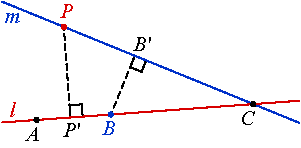
\includegraphics[height=.85in]{main/Sylvester_Gallai_Kelly_proof}
\vskip-8pt
\caption{Construction for the Sylvester-Gallai theorem.}
\label{Fig4-S}
\end{figure}
%
in $\PP^2_\CC$ passes through a third flex; but
such a configuration is not possible in $\PP^2_\RR$. Prove:

\begin{theorem}[Sylvester--Gallai theorem]
In any finite set  $\Gamma \subset \PP^2_\RR$ there are three 
noncollinear points unless $\Gamma$ is contained in a line.
\unif
\end{theorem}

Hint (following Leroy Milton Kelly): 
\index{Kelly, Leroy Milton}%
We may assume that $\Gamma\subset \RR^2` `$. Choose a pair $P,L$ consisting of a point $P\in\Gamma$ and line $\ell$ containing at least 2 of the points of $\Gamma$, but not $P$, such that the distance from $L$ to $p$ is
minimal among such pairs. If there were at least 3 points of $\Gamma$
on $L$ then, considering  
Figure~\ref{Fig4-S},
show that
there is a point of $\Gamma$ and a line $L'$ violating the minimal distance hypothesis.
\end{exercise}
\input footer.tex
